% mainfile: ../../main.tex
\chapter{Monte Carlo and \texorpdfstring{\acrshort{gksl}}{GKSL} master equation simulations}\label{ch:app:ff:time_domain_methods}
\section{Validation of \texorpdfstring{\acrshort{qft}}{QFT} fidelities}\label{sec:app:ff:time_domain_methods:qft_validation}
In this section, we perform \gls{gksl} master equation and \gls{mc} simulations to verify the fidelities predicted for the \gls{qft} circuit in the main text.
We focus on noise exclusively on the third qubit, entering through the noise operator $B_\alpha\equiv\sigma_y\gth{3}$.

\todo{this}
We assemble the \gls{qft} circuit discussed in the main text from a minimal gate set consisting of three atomic gates, $\mathbb{G} = \lbrace\mr{X}_{i}(\flatfrac{\pi}{2}),\mr{Y}_{i}(\flatfrac{\pi}{2}),\mr{CR}_{ij}(\flatfrac{\pi}{2^3})\rbrace$ on or between qubits $i$ and $j$.
We consider a simple model involving four single-spin qubits with in-phase (I) and quadrature (Q) single-qubit control and nearest neighbor exchange coupling so that the control Hamiltonian reads
\begin{equation}\label{eq:app:ff:control_hamiltonian:qft}
    H_\mr{c}(t) = \sum_{\langle i,j\rangle} I_i(t)\sx^{(i)} + Q_i(t)\sy^{(i)} + J_{ij}(t)\sz^{(i)}\otimes\sz^{(j)}
\end{equation}
where $\sigma_\alpha^{(i)}$ is the trivial extension of the Pauli matrix $\sigma_\alpha$ of qubit $i$ to the full tensor product Hilbert space.
For simplicity, we assume periodic boundary conditions so that qubits 1 and 4 are nearest neighbors as well.
Similarly, we define the noise Hamiltonian as
\begin{equation}\label{eq:app:ff:noise_hamiltonian:qft}
H_\mr{n}(t) = \sum_{\langle i,j\rangle} b_{I}(t)\sx^{(i)} + b_{Q}(t)\sy^{(i)} + b_{J}(t)\sz^{(i)}\otimes\sz^{(j)}
\end{equation}
with the noise fields $b_{\alpha}(t)$ for $\alpha\in\{I,Q,J\}$.

To validate the fidelity for white noise, we use a \gls{gksl} master equation~\cite{Lindblad1976,Gorini1976} in superoperator form.
We represent linear maps $\mc{A}: \rho\rightarrow\mc{A}(\rho)$ by matrices in the \gls{ptm} representation as (see \citer{Hangleiter2021} for more details)
\begin{equation}
    \mc{A}_{ij} \coloneqq \tr(\sigma_i\mc{A}(\sigma_j))
\end{equation}
and operators as column vectors (\ie, generalized Bloch vectors) as
\begin{equation}\label{eq:app:ff:bloch_vector}
    \rho_i \coloneqq \tr(\sigma_i\rho),
\end{equation}
allowing us to write the Lindblad equation
\begin{equation}\label{eq:app:ff:lindblad:hilbert}
\dv{t}\rho(t) = -\i\comm{H(t)}{\rho(t)} + \sum_\alpha \gamma_\alpha\left(L_\alpha\rho(t) L_\alpha\adjoint - \frac{1}{2}\acomm{L_\alpha\adjoint L_\alpha}{\rho(t)}\right)
\end{equation}
as a linear differential equation in matrix form,
\begin{equation}\label{eq:app:ff:lindlbad:liouville}
\dv{t}\rho_i(t) = \sum_j\left(-\i\mc{H}_{ij}(t)+ \sum_\alpha \gamma_\alpha \mc{D}_{\alpha, ij}\right)\rho_j(t).
\end{equation}
Here, $\mc{H}_{ij}(t) = \tr(\sigma_i\comm{H(t)}{\sigma_j})$ and $\mc{D}_{\alpha, ij} = \tr(\sigma_i L_\alpha\sigma_j L_\alpha\adjoint - \frac{1}{2}\sigma_i \acomm{L_\alpha\adjoint L_\alpha}{\sigma_j})$.
By setting $L_\alpha\equiv\sigma_y\gth{3}$ as well as $\gamma_\alpha\equiv\flatfrac{S_0}{2}$ with $S_0$ the amplitude of the one-sided noise \gls{psd} so that $S(\omega) = S_0$, we can compare the fidelity obtained from the filter functions to that from the explicit simulation of \cref{eq:app:ff:lindlbad:liouville}.
The latter is computed as $\avgfid = d^{-2}\tr(\mc{Q}\adjoint\mc{U})$, where $\mc{Q}$ is the superpropagator due to the Hamiltonian evolution alone (\ie, the ideal evolution without noise).

For the Monte Carlo simulation, we explicitly generate time traces of $b_Q(t)$ (\cf \cref{eq:app:ff:noise_hamiltonian:qft}) by drawing pseudo-random numbers from a distribution whose \gls{psd} is $S(f) = \flatfrac{S_0}{f}$.
To do this, we draw complex, normally distributed samples in frequency space (\ie white noise), scale it with the square root of the \gls{psd}, and finally perform the inverse Fourier transform.
We choose an oversampling factor of 16 so that the time discretization of the simulation is $\Delta t_\mr{MC} = \flatfrac{\Delta t}{16} = \qty{62.5}{\pico\second}$ ($\Delta t = \qty{1}{\nano\second}$ is the time step of the pulses used in the \gls{ff} simulation), leading to a highest resolvable frequency of $\fmax = \qty{16}{\giga\hertz}$.
Conversely, we increase the frequency resolution by sampling a time trace longer by a given factor, giving frequencies below \fmin (\qty{16}{\kilo\hertz} for pink, \qty{0}{\hertz} for white noise) weight zero, and truncating it to the number of time steps in the algorithm times the oversampling factor.
This yields a time trace with frequencies $f\in [\fmin, \fmax]$ and a given resolution (we choose $\df = \qty{160}{\hertz}$).
% TODO: check parameters
For reference, we show the fidelity filter functions for the circuit with and without echo pulses in this frequency band in \cref{fig:app:qft_ff}.

We then proceed to diagonalize the Hamiltonian $H(t) = H_c(t) + H_n(t)$ and compute the propagator for one noise realization as
\begin{equation}\label{eq:app:ff:mc_propagator}
U(t) = \prod_g V\gth{g}\exp\lbrace -\i\Omega\gth{g}\Delta t_\mr{MC}\rbrace V^{(g)\dagger},
\end{equation}
where $V\gth{g}$ is the unitary matrix of eigenvectors of $H(t)$ during time segment $g$ and $\Omega\gth{g}$ the diagonal matrix of eigenvalues.
Finally, we obtain an estimate for the average gate fidelity \avgfid from the entanglement fidelity \entfid as
\begin{equation}
    \ev{\avgfid} = \ev{\frac{d\entfid + 1}{d+1}} = \ev{\frac{\abs{\tr(Q\adjoint U(\tau))}^2 + d}{d(d+1)}}.
\end{equation}
Here, $Q\equiv\Uc(t=\tau)$ is the noise-free propagator at time $\tau$ of completion of the circuit and $\ev{\placeholder}$ denotes the ensemble average over $N$ Monte Carlo realizations of \cref{eq:app:ff:mc_propagator}, \ie, $\ev{A}=N\inverse\sum_{i=1}^N A_i$.
The standard error of the mean can be obtained as $\sigma_{\ev{\avgfid}} = \sigma_{\avgfid} / \sqrt{N}$ with $\sigma_{\avgfid}$ the standard deviation over the Monte Carlo traces.

\begin{figure}
    \centering
    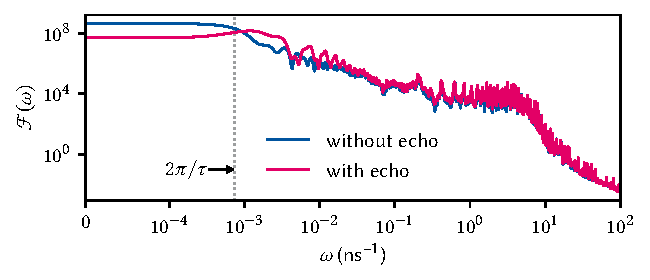
\includegraphics{img/pdf/filter_functions/qft_filter_function_Y3}
    \caption[\imgsource{img/py/filter_functions/quantum_fourier_transform.py}]{
        Filter functions for noise operator $\sigma_y^{(3)}$ for the \gls{qft} circuit without (blue) and with (magenta) additional echo pulses.
        Introducing the echoes shifts spectral weight towards higher frequencies, reducing the DC level of the filter function by two orders of magnitude and thus leading to an improved fidelity for \oneoverf noise.
    }
    \label{fig:app:qft_ff}
\end{figure}
\begin{table*}
    \centering
    \renewcommand\arraystretch{1.25}
    \caption{Infidelities $\avginfid = 1-\avgfid$ of the \gls{qft} circuit due to noise on $\sigma_y^{(3)}$. \Gls{mc} values are given with the standard error of the mean for $N=1008$. We included frequencies in the range of $\omega\in [0, 100]\,\unit{\per\nano\second}$ for white noise, and $\omega\in [\qty{100}{\per\milli\second}, \qty{100}{\per\nano\second}]$ for pink noise. Prefactors in the power law $S(\omega)= A\omega^\alpha$ are \qty{2e-6}{\per\nano\second} and \qty{1e-9}{\per\nano\second\squared}, respectively.}
    \label{tab:app:fidelities}
    \begin{tabular}{l *{4}{r}}
        \toprule
        & \multicolumn{2}{c}{\textsc{White noise}} & \multicolumn{2}{c}{$\flatfrac{1}{f}$ \textsc{noise}} \\
        \cmidrule(lr){2-3}\cmidrule(lr){4-5}
        \textsc{Method} & \textsc{Without echo} & \textsc{With echo} & \textsc{Without echo} & \textsc{With echo} \\
        \midrule
        \acrshort{gksl} & \num{8.38e-3}         & \num{8.38e-3}      & ---                   & ---               \\
        \acrshort{mc}   & \num{8.22(24)e-3}     & \num{8.34(23)e-3}  & \num{8.53(28)e-3}     & \num{2.84(10)e-3} \\ %2021-07-20_17-30-32
        \acrshort{ff}   & \num{8.34e-3}         & \num{8.40e-3}      & \num{8.34e-3}         & \num{3.02e-3}     \\ %2021-07-20_16-41-17
        \bottomrule
    \end{tabular}
\end{table*}

\Cref{tab:app:fidelities} compares the infidelities $\infid=1-\fid$ from \gls{gksl} and \gls{mc} simulations to the filter function predictions following \cref{eq:ff:infidelity:ent}.
Note that the precise value of the filter function result depends quite sensitively on the frequency sampling due to the sharp peaks in the gigahertz range (\cref{fig:app:qft_ff}).
As the table shows, both the \gls{gksl} and the \gls{mc} calculations agree well with the predictions made by our filter-function formalism.